\documentclass{standalone}
\usepackage[centertags]{amsmath}
\usepackage{latexsym}
\usepackage{amsfonts}
\usepackage{amssymb}
\usepackage{amsthm}
\usepackage{newlfont}
\usepackage{enumerate}
\usepackage{makeidx}
\usepackage{tikz}
\usetikzlibrary{backgrounds,intersections}
\begin{document}
        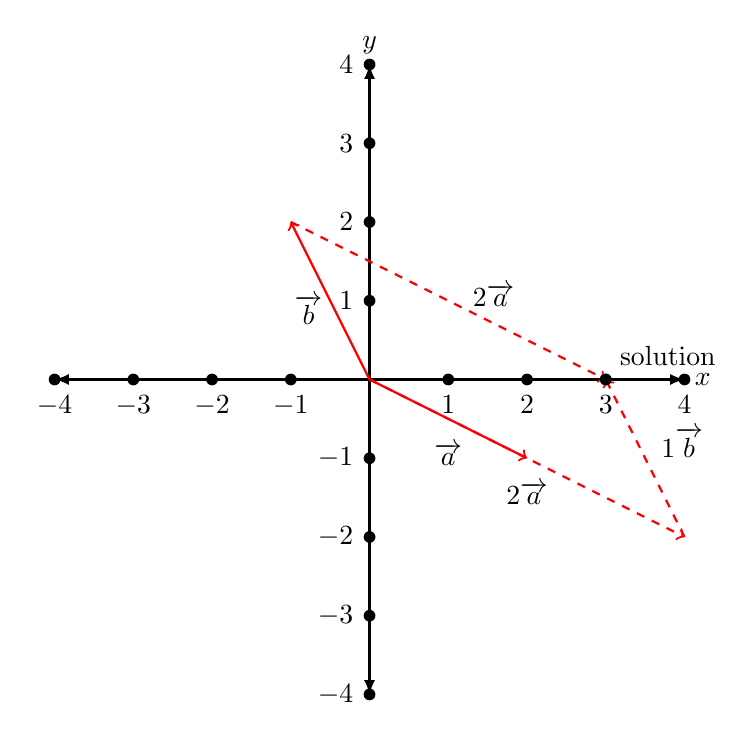
\begin{tikzpicture}
        \draw[thick,latex-latex] (-4,0) -- (4,0)node[right]{$x$};
        \draw[thick,latex-latex] (0,-4) -- (0,4)node[above]{$y$};
        \foreach \x in {-4,-3,-2,-1,1,2,3,4}{
            \node[fill,circle,inner sep=1.5pt,label=below:$\x$] at (\x,0) {};
            \node[fill,circle,inner sep=1.5pt,label=left:$\x$] at (0,\x) {};
        }
        \draw[red,thick,->] (0, 0) -- (2,-1)
	node[pos=0.5,black,below,yshift=-0.5em] {$\overrightarrow{a}$};
        \draw[red,thick,->] (0, 0) -- (-1,2)
	node[pos=0.6,black,below,xshift=-0.5em] {$\overrightarrow{b}$};
        \draw[red,thick,dashed,->] (0, 0) -- (4,-2)
	node[pos=0.5,black,below,yshift=-0.5em] {2$\overrightarrow{a}$};
        \draw[red,thick,dashed,->] (4, -2) -- (3,0)
	node[pos=0.6,black,right,xshift=0.5em] {1$\overrightarrow{b}$};
        \draw[red,thick,dashed,->] (-1, 2) -- (3,0)
	node[pos=0.6,black,above,xshift=0.5em] {2$\overrightarrow{a}$};
	\node[fill,circle,inner sep=1.5pt,label=above right:solution] at (3,0) {};

        \end{tikzpicture}
\end{document}
